\section{Détail du sujet de stage}
\label{sec:sujet}
Le sujet de mon stage était ainsi formulé : \og Intégration de tests de sécurité dans le processus d'intégration continue, et développement Java selon les besoins de l'entreprise. \fg Nous avions convenu, lors de l'entretien d'embauche, que mon travail serait également réparti entre ces deux aspects.

En pratique, cela a représenté plusieurs projets différents et une intervention en tant que consultant.

\subsection{Sécurité \& CI}
La partie la plus précisément définie de mon stage : Alter Frame dispose d'un système d'intégration continu qui, à mon arrivée, incorporait de l'analyse qualité et la compilation du code à chaque \textit{push} sur leur plateforme git.

Mon travail serait donc d'incorporer un aspect sécurité à la configuration déjà existante, de manière à obtenir le processus du graphique~\ref{fig:ci_flow}.

Éléments à implémenter :
\begin{itemize}[label=$\bullet$]
	\item analyse dynamique, uniquement dans le cas d'application web, en automatisant des tests de sécurité avec ZAP ;
	\item analyse statique, si le temps le permettait, en réutilisant les analyses de code \textit{via} Sonar déjà en place et les affinant d'un point de vue sécurité.
\end{itemize}
Ces tâches de départ dépendent de plusieurs autres qui faisaient, de fait, également partie de mon sujet de stage. Réaliser des analyses de sécurité contre les applis web d'Alter Frame impliquaient que celles-ci soient accessibles en ligne, au minimum sur un serveur privé pour les besoins du développement. Automatiser ce déploiement, et idéalement pouvoir l'étendre pour réaliser une livraison dans certaines conditions (telles qu'un \textit{push} tagué), devrait donc être la première étape à réaliser, avant d'ensuite programmer les tests, ZAP ayant le bon goût d'être très finalement contrôlable par des APIs dans plusieurs langages\cite{zap_api} et en ligne de commande\cite{zap_cli}\cite{zap_cli_wrapper}.

Par ailleurs, si la partie analyse statique devait se réaliser, cela impliquait d'apprendre le fonctionnement des plugins sonars et comment étendre les règles créées par défaut par l'analyseur, pour ensuite à proprement parler isoler des problématiques de sécurité qui peuvent être adressées et les faire vérifier.

\begin{figure}
	\centering
	\caption{Déroulement du processus d'intégration continue}
	\label{fig:ci_flow}
	\frame{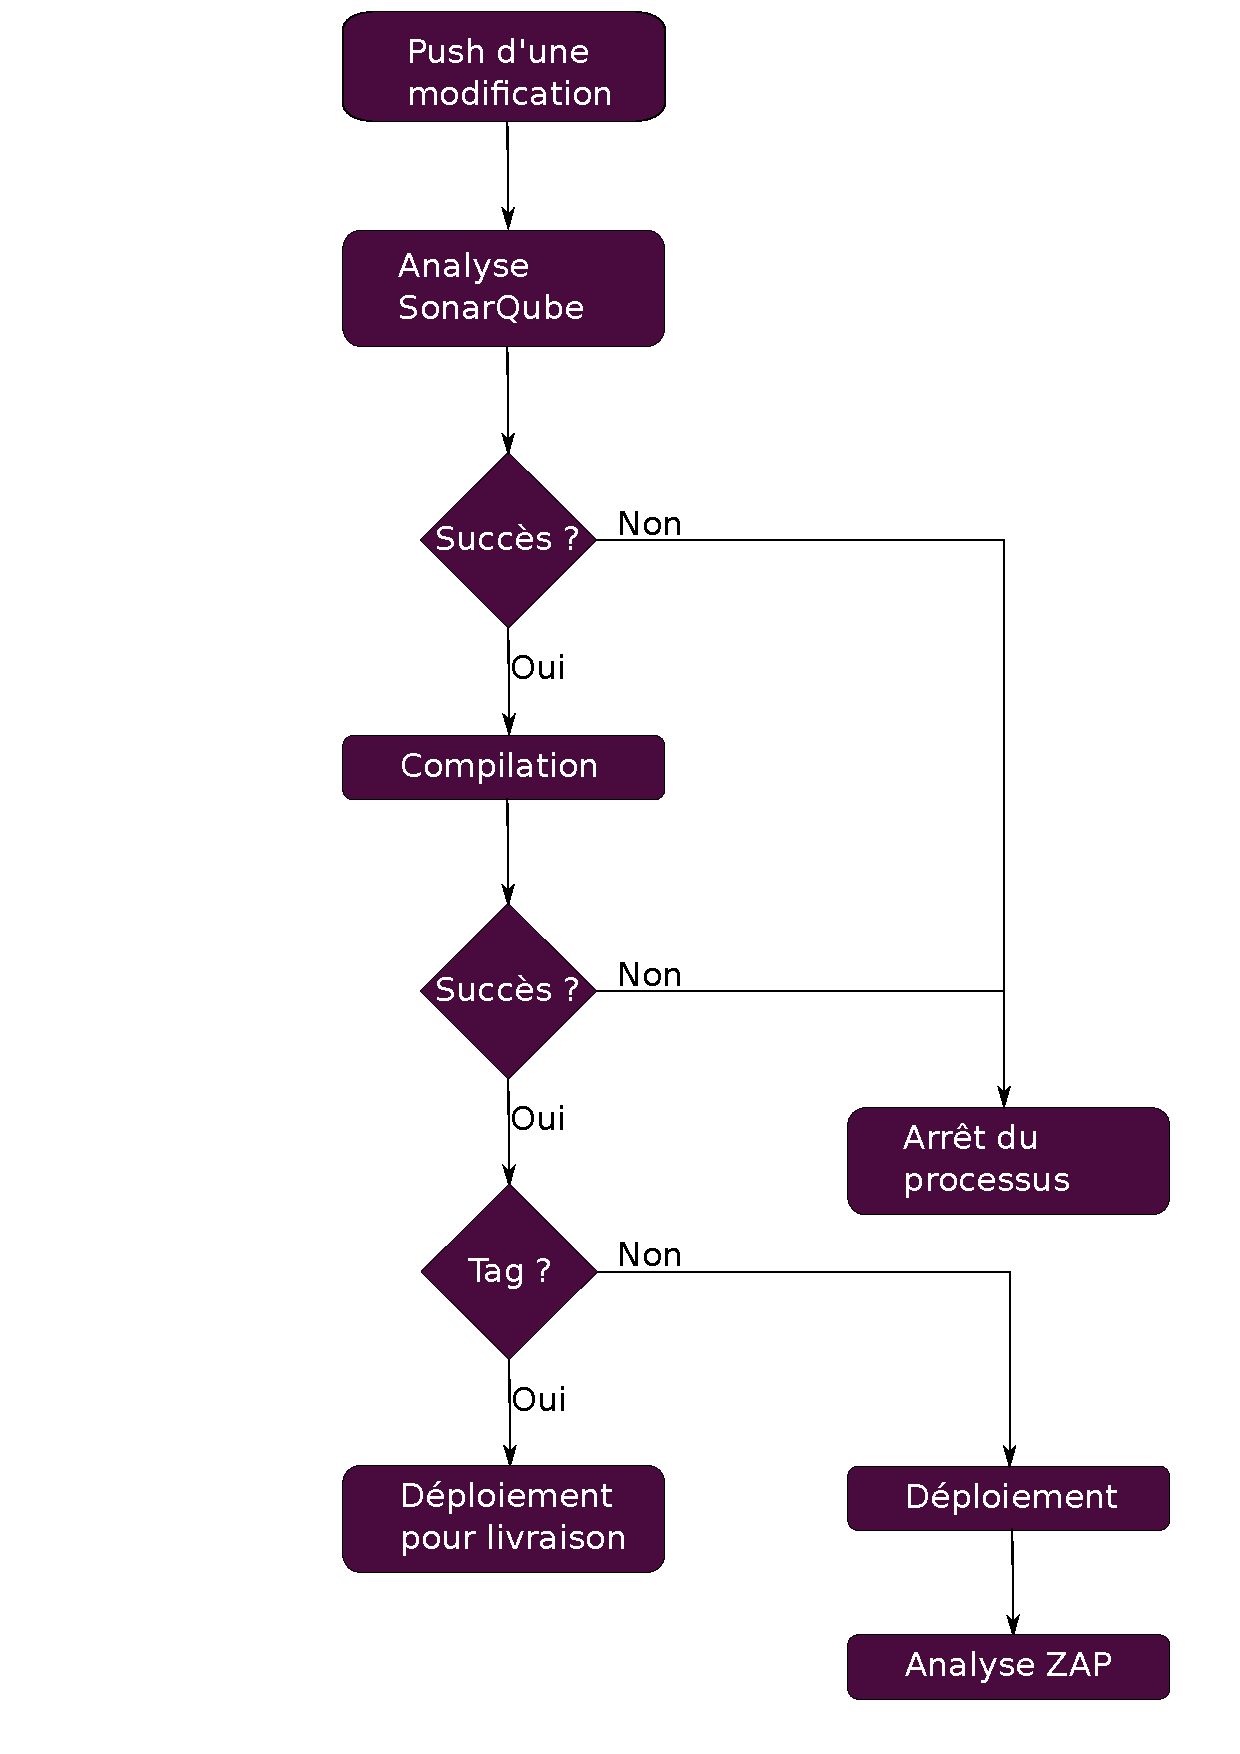
\includegraphics[width=\textwidth]{images/CI_flow.pdf}}
\end{figure}

\subsection{Développement Java}
L'aspect Java, dans mon stage, était plus flou dans la mesure où il était sujet aux projets qui seraient en cours et en besoin de soutien au moment de mon arrivée dans l'entreprise. En pratique, cela a été majoritairement du développement sur un projet de gestions de tests sur des voitures, pour un constructeur automobile, ainsi que des interventions ponctuelles sur plusieurs autres projets destinés au même client.

\subsection{Interventions en fonction du besoin}
De même que le développement Java, cette partie de mon travail était sujette à évolution en fonction du besoin. En fin de stage, elle a pris la forme d'un audit technique pour une compagnie d'assurance qui souhaitait améliorer son service d'Intranet, tant d'un point de vue sécurité que qualité de code ou performances d'exécution.

Durant cet audit j'ai eu à gérer une partie de l'aspect sécurité de notre intervention, et une partie de l'aspect performance, cela au cours d'une mission de 3 jours chez le client.